\documentclass[10pt]{article}
\usepackage{array, xcolor, lipsum, bibentry}
\usepackage[margin=3cm]{geometry}
\usepackage[english,russian]{babel}
\usepackage[utf8]{inputenc}
\usepackage{graphicx}
\usepackage{url}

\title{\bfseries\Huge Oleg N. Babichev}
\author{babichev.oleg.n@gmail.com}
\date{}


\definecolor{lightgray}{gray}{0.8}
\newcolumntype{L}{>{\raggedleft}p{0.14\textwidth}}
\newcolumntype{R}{p{0.8\textwidth}}
\newcommand\VRule{\color{lightgray}\vrule width 0.5pt}

\begin{document}
\maketitle
\vspace{1em}
\begin{minipage}[ht]{0.48\textwidth}
Pervomayskaya st. 15-45\\
Dolgoprudny 141701\\
Moscow region\\
Russia
\end{minipage}
\begin{minipage}[ht]{0.48\textwidth}
July 20th, 2016\\
+7 925 724 61 77
\end{minipage}

\smallskip

\begin{minipage}[ht]{0.48\textwidth}
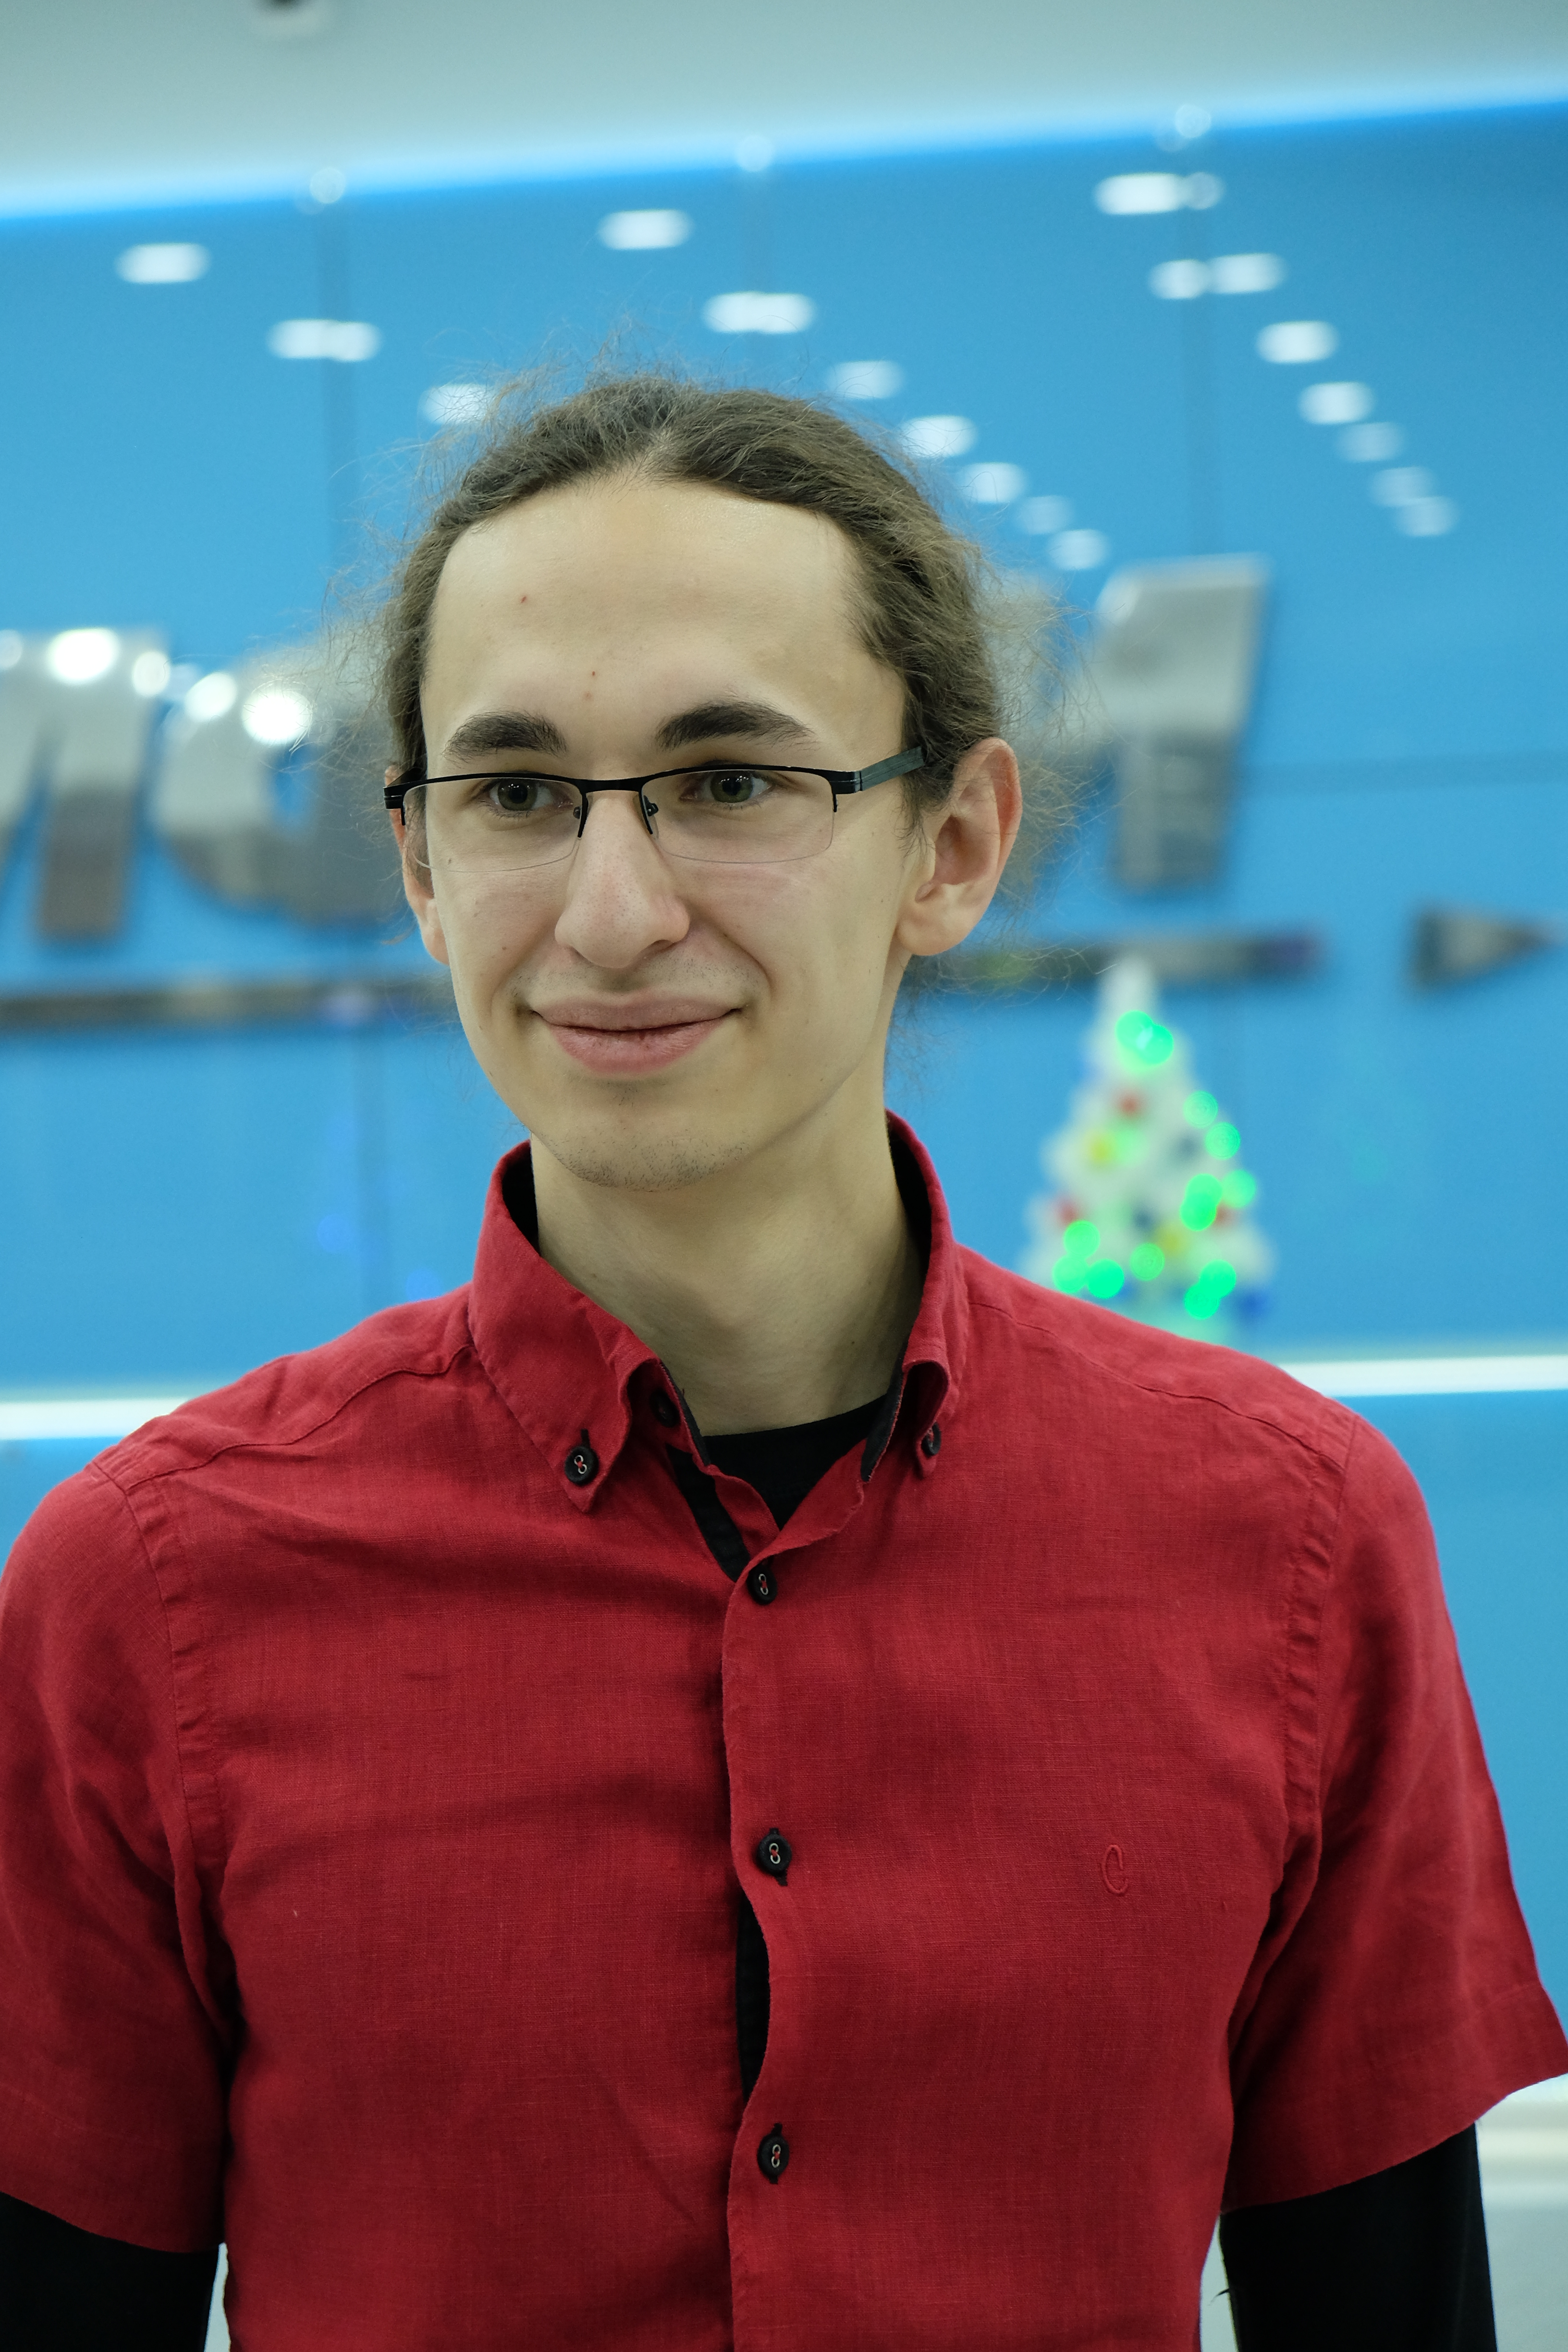
\includegraphics[width=5cm]{photo}
\end{minipage}

\vspace{20pt}

%\section*{Objective}
%Curriculum vitae

\section*{Professional Experience}
\begin{tabular}{L!{\VRule}R}
2013--2015 & {\bf Intel platform simulator developer (Intern),} \textit{Intel corporation, Moscow}\\
2015--today&{\bf Android developer,} \textit{Sberbank-Technology, Moscow}\\
\end{tabular}

\section*{Education}
\begin{tabular}{L!{\VRule}R}
2015--2017 & {\bf MSc in Applied Mathematics and Informatics,}  \textit{Moscow Institute of Physics and Technology},\\
		& \textit{Department}: Department of Innovation and High Technology,\\
		&\textit{Subject}: Social network analysis of email communication in company\\
		&\textit{Supervisor}: Associate professor Zvonov Denis\\
2011--2015 & {\bf BSc in Applied Mathematics and Physics}, \textit{Moscow Institute of Physics and Technology},\\
		& \textit{Department}: Department of Radio Engineering and Cybernetics\\
		&\textit{Subject}: Research of performance of full-system simulator Simics\\
		&\textit{Supervisor}: Associate professor Stepin Andrey
\end{tabular}

\section*{Languages}
\begin{tabular}{L!{\VRule}R}
Russian&Mother tongue\\
{English}&{Intermediate}\\
\end{tabular}

\section*{Programming skills}
\begin{tabular}{L!{\VRule}R}
Java & SE, Spring, RxJava \\
Android Developing & MVP, Dagger \\
Python & Simulator device modelling, data analysis, pandas, django web developing,  \\
C, C++ & Simulator device modelling \\
JavaScript & ios developing with react-native, web \\
Matlab & image processing course \\
BigData & hadoop map reduce course \\
\end{tabular}

\section*{Other skills}
\begin{tabular}{L!{\VRule}R}
OS & Linux, Windows, MacOs\\
CVS & git, svn \\
\end{tabular}

\section*{Coursera cources}
\begin{itemize}
	\item Mathematics and Python for data analysis: part 1.
	\item Programming Mobile Applications for Android Handheld Systems: Part 1
\end{itemize}

\section*{My profiles}
\begin{itemize}
	\item LinkedIn: \url {https://www.linkedin.com/in/oleg-babichev-5b019210b}
	\item GitHub: \url {https://github.com/obabichev/} (old: \url{https://github.com/ochuikin})
	\item FaceBook: \url {http://facebook.com/obabichev}
\end{itemize}


\bibliographystyle{plain}
\nobibliography{publication}

%\section*{Books}
%\begin{tabular}{L!{\VRule}R}
%2015&\bibentry{Babichevs}
%\end{tabular}


\end{document} 